\documentclass[tikz, border=5pt]{standalone}
\usetikzlibrary{arrows.meta, shapes, positioning, decorations.pathmorphing, patterns}

\tikzset{
  spring/.style = {
    decoration = {aspect=0.3, segment length=2mm, amplitude=2.5mm, coil, pre length=4mm, post length=3mm},
    decorate
  }
}

\begin{document}
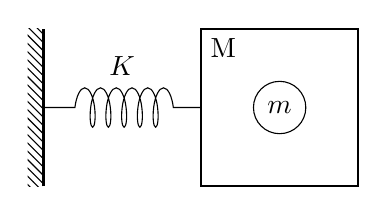
\begin{tikzpicture}

  %% TORA System

  % Wall
  \draw[thick] (-5,0) -- (-5,2);
  \fill[pattern = north west lines] (-5,0) rectangle (-5.2,2);

  % Spring
  \draw[spring] (-5,1) -- (-3,1) node[midway, above, yshift=8] {\(K\)};

  % Cart
  \draw[thick] (-3,0) rectangle (-1,2);
  \node[below right] at (-3, 2) {M};

  % Pendulum
  \node[draw, circle, minimum size=0.5cm] (pendulum) at (-2,1) {\(m\)};

\end{tikzpicture}
\end{document}
